\pagestyle{plain}  % kvuli cislovani

\chapter{Sada nástrojů}

\todo[inline, color=blue!30]{TODO: Rychlý úvod do všech nástrojů. Rozebrat hlavně mm-evocat, protože ten je základem návrhu. }


\section{MM-cat}

MM-cat framework je navržený tak, aby řešil složitosti spojené s návrhem a správou multi-modelových databází. Jeho hlavním úkolem je modelování multi-modelových schémat a jejich mapování na příšlušné Systémy řízení bází dat (SŘBD). Slouží i jako základ pro rozšíření o složitější úkoly.

Typickým scénářem použití je vytvoření ER (entity-relationship) schématu uživatelem. Takové schéma je pak automaticky převedeno do jednotné kategorické reprezentace, která umožňuje namapování na kombinaci SŘBD. Díky specifikaci schématu je vytvořen skript s příkazy CREATE, které se aplikují na přiřazené SŘBD. Uživatel může následně dál upravovat ER diagram, nebo provádět SELECT dotazy.

Na ukázce uživatelského rozhraní (Obrázek \ref{obr01:mm-cat}) je výsledek typického scénáře rozebraného v předchozím odstavci. Na levé straně je uživatelem vytvořený ER diagram, na straně pravé pak jeho kategorická reprezentace. Na pravé straně ještě stojí za povšimnutí panel s přístupovými cestami (značené oranžově) a CREATE příkaz.

\begin{figure}[htb]
  \centering
  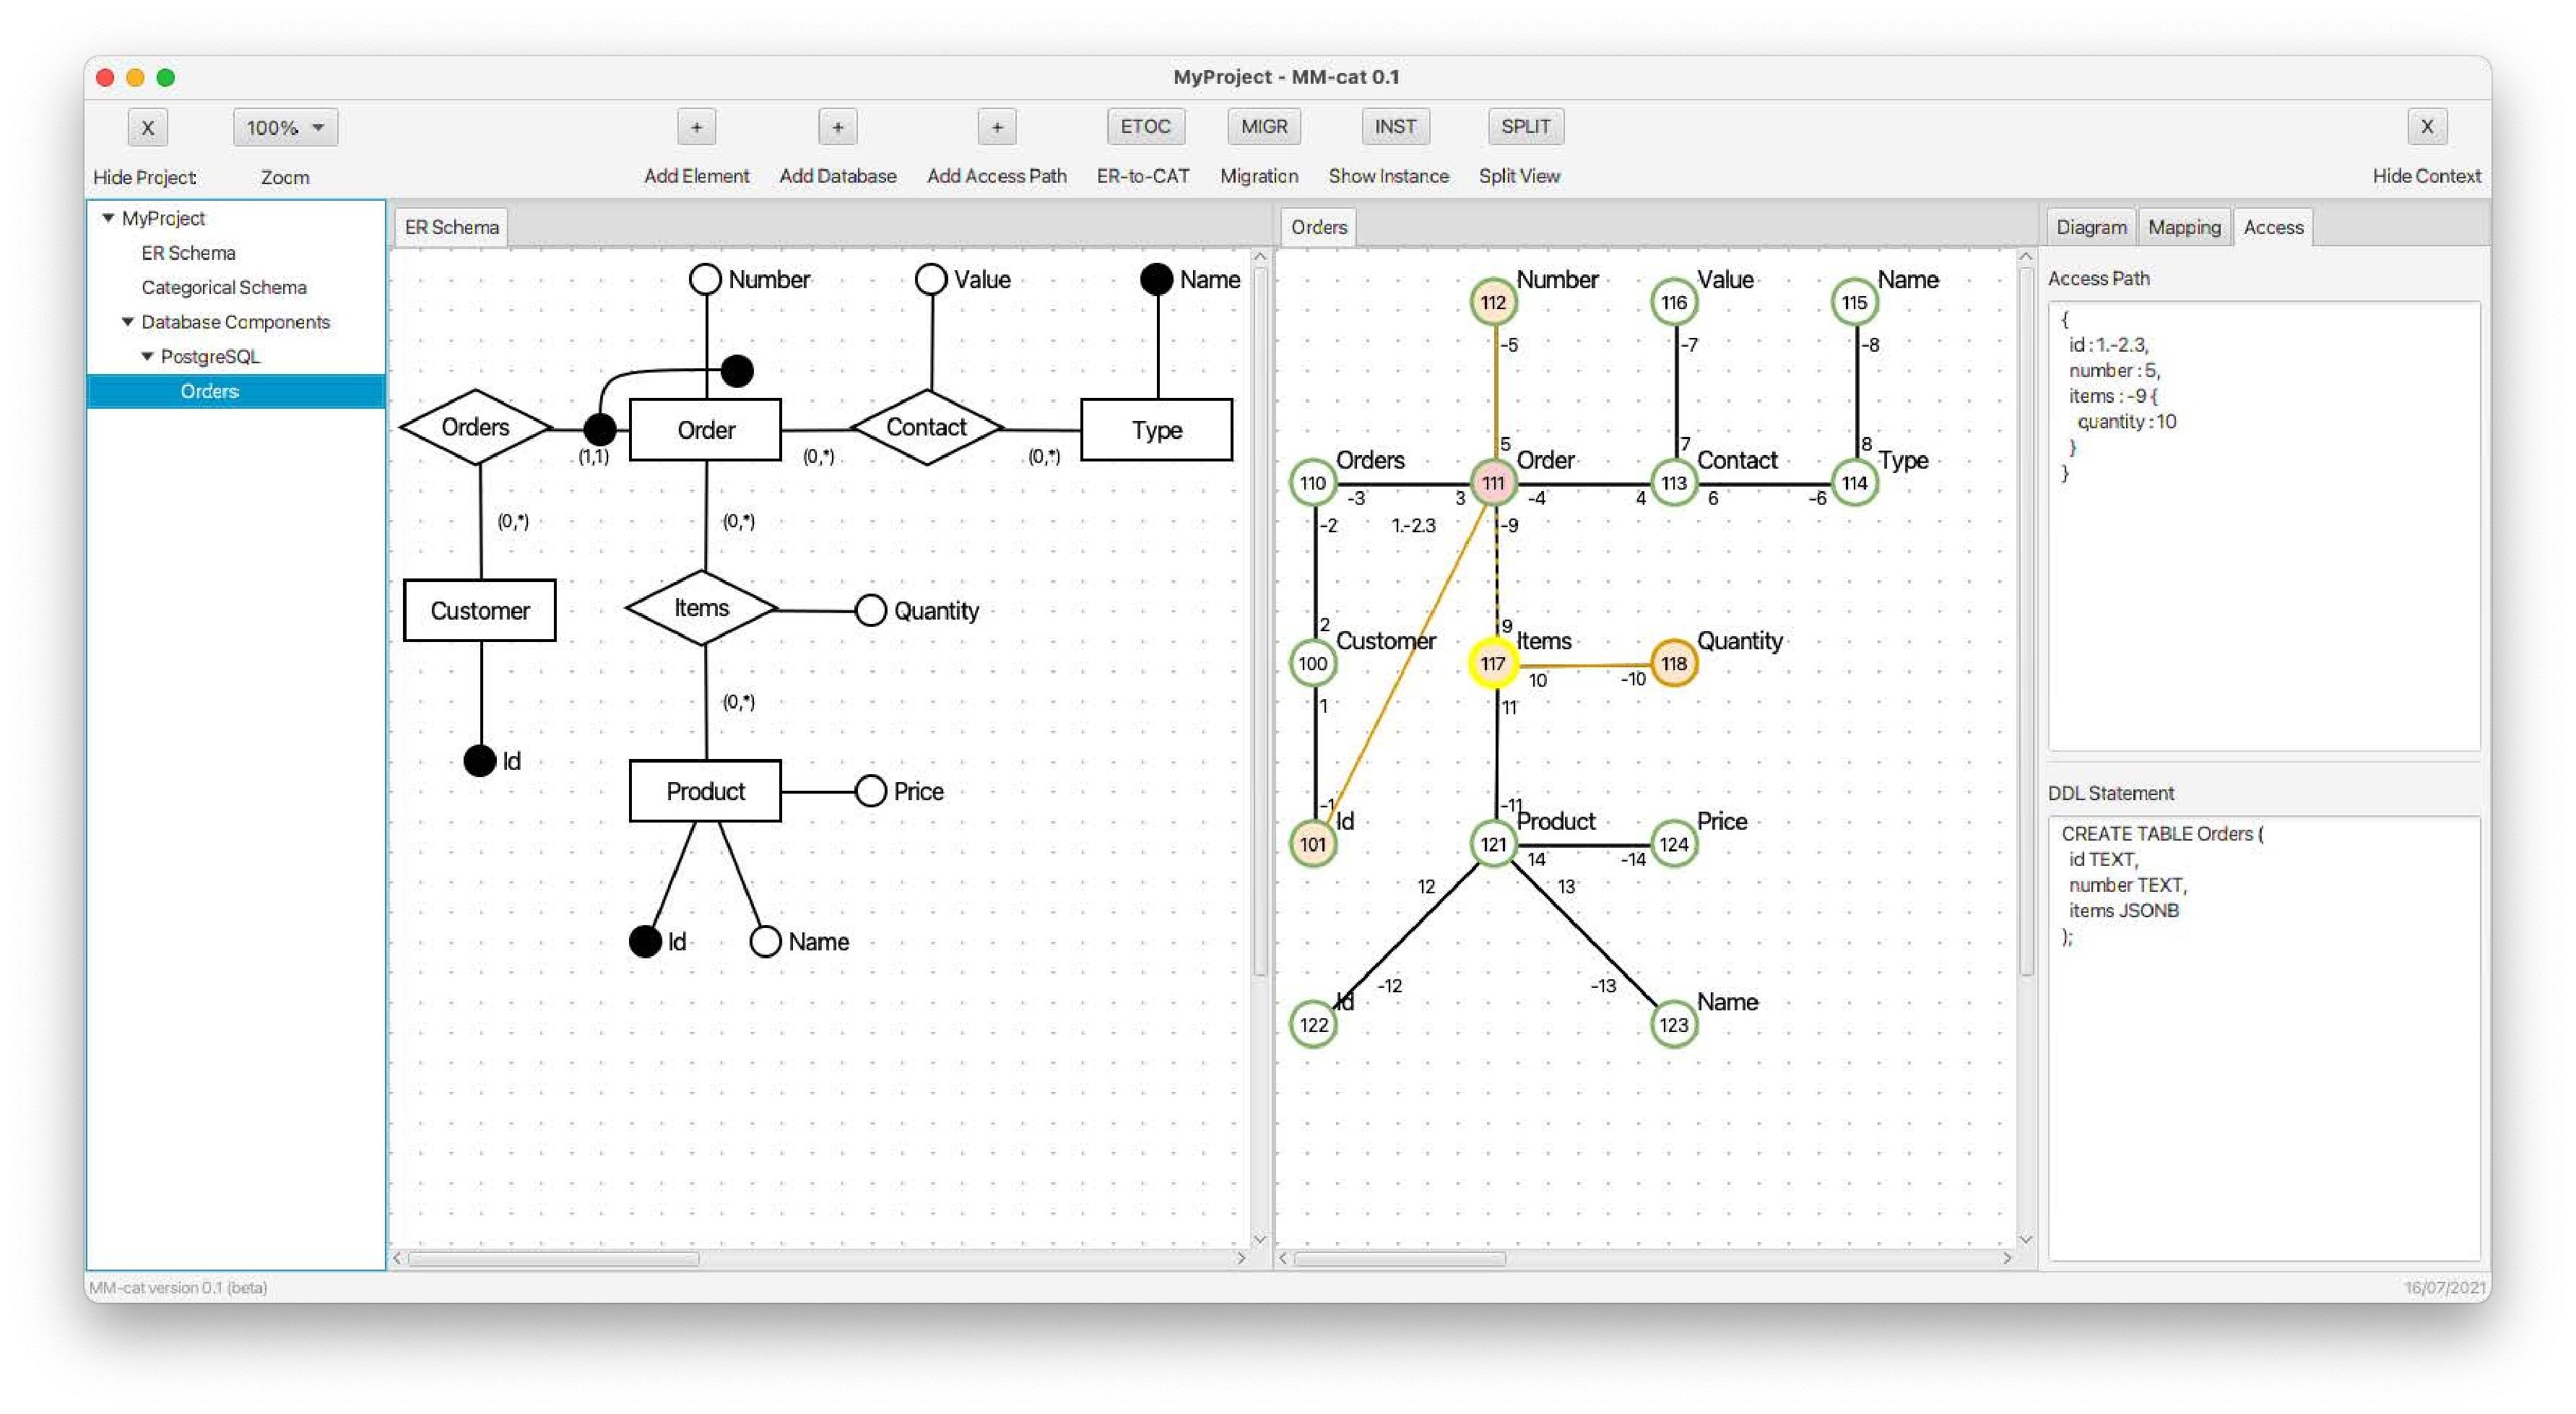
\includegraphics[height=75mm]{../img/mm-cat}
  \caption{Ukázka uživatelského rozhraní nástroje MM-cat.}
  \label{obr01:mm-cat}
\end{figure}

Další možnosti použití, i podrobnější popis nástroje, lze nalézt v článku \citet{MMcat}.


\section{MM-infer}

Ne všechna data mají předem definované schéma. Nástroj MM-infer se snaží schéma zpětně zrekonstruovat z již uložených multi-modelových dat. Je schopen odhalit intra- a inter-modelové reference a překrývání modelů. Zároveň nástroj umí efektivně zpracovávat velké množství dat.

MM-infer podporuje tři druhy SŘBD, vybrané tak, aby bylo pokryto co nejvíc funkcí takových systémů. PostreSQL byl vybraný jako zástupce schema-full, relační SŘBD. Neo4j reprezentuje schema-less a MongoDB obojí. 

Rozhraní aplikace nás provede hned několika kroky, jejichž výsledkem je globální schéma pro vybranou množinu SŘBD. Uživatel musí nejdřív takové SŘBD vybrat (Obrázek \ref{obr01:mm-infer-load-database}). V levém panelu je osa ukazující již splněné a následující kroky, pro lepší orientaci v procesu.

\begin{figure}[htb]
  \centering
  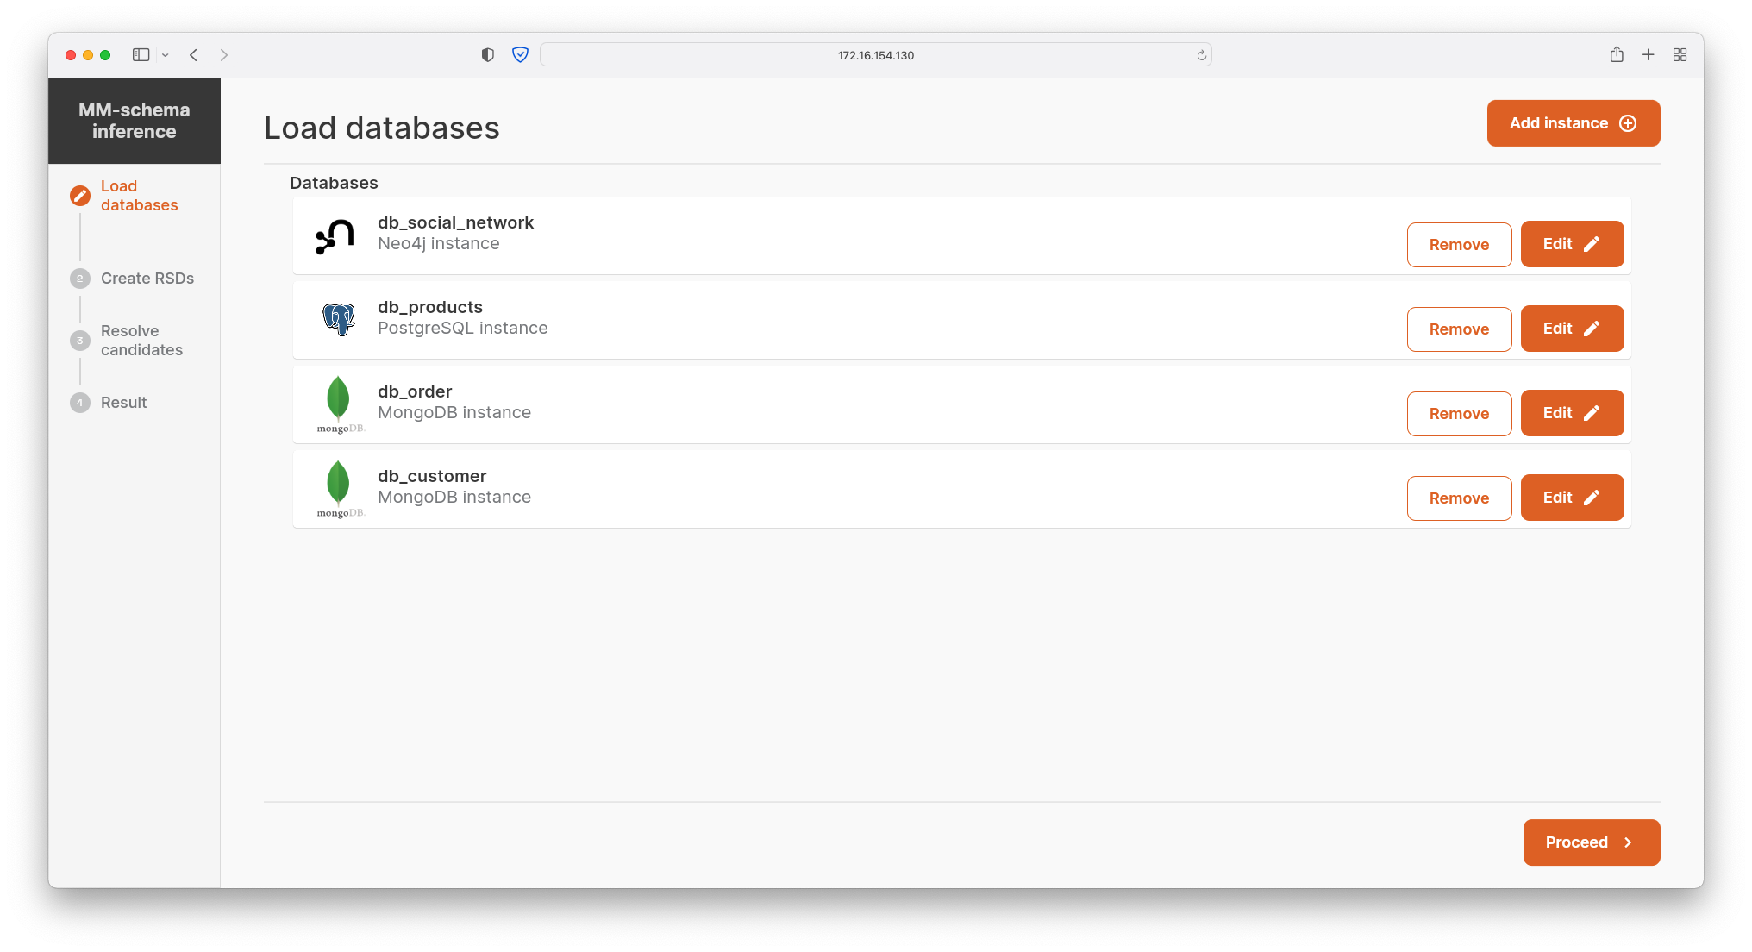
\includegraphics[height=75mm]{../img/mm-infer-load-database}
  \caption{Načtení databází v nástroji MM-infer.}
  \label{obr01:mm-infer-load-database}
\end{figure}

Podle vybraných databází a dalších parametrů je vytvořen RSD (Record Schema Description), sjednocující reprezentace. Po automatickém načtení je pak předána ruka uživateli, který kontroluje navržené kandidáty. Výsledkem je vizualizace globálního schématu (Obrázek \ref{obr01:mm-infer-result}).

\begin{figure}[htb]
  \centering
  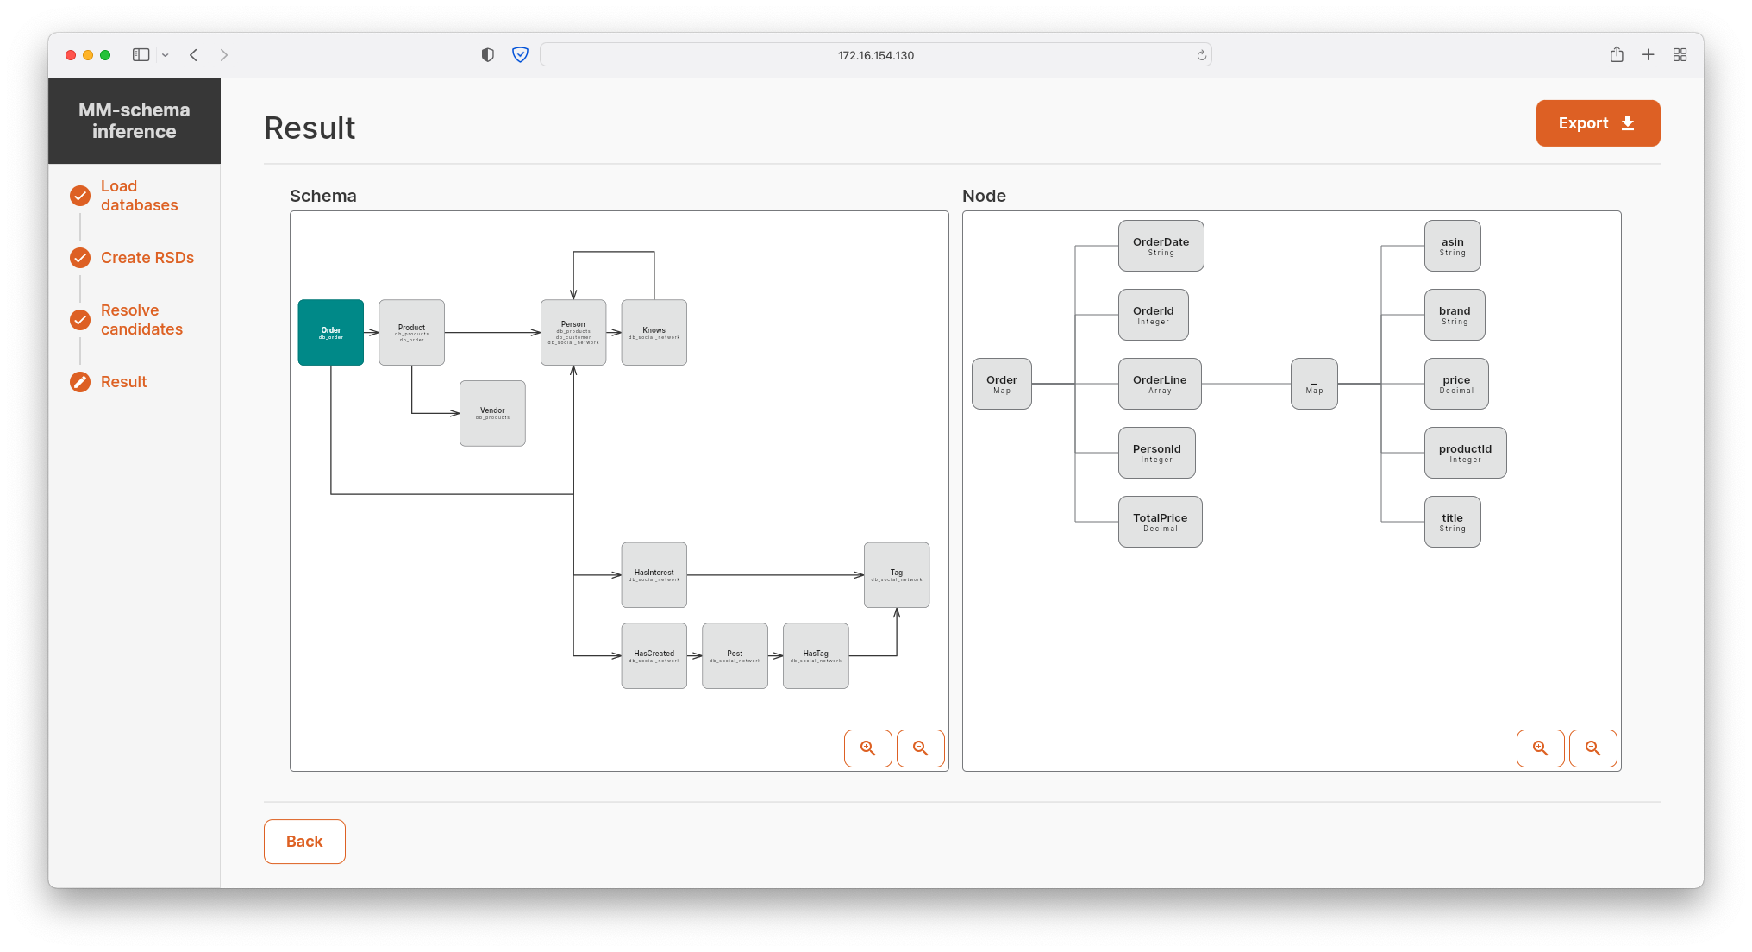
\includegraphics[height=75mm]{../img/mm-infer-result}
  \caption{Vizualizace globálního schématu v nástroji MM-infer.}
  \label{obr01:mm-infer-result}
\end{figure}

Aplikace příjemně provádí uživatele všemi potřebnými kroky. Nemá zbytečně příliš různých grafických prvků, které by uživatele zahlcovaly. Stejně jako mm-cat využívá dvou oken pro diagramy vedle sebe.

Další informace o návrhu a možnostech použití aplikace lze nalézt v \citet{MMinfer}.

\section{MM-evocat}

MM-evocat je nástroj pro modelování a správu evoluce v multi-modelových datech. Řeší případy, kdy se struktura dat v čase mění tak, aby například vyhovovala novým uživatelským požadavkům. Takové změny jsou pak propagovány napříč definovanými modely a datovými instancemi.

Umožňuje vytvářet kategorický model, umí ho dekomponovat a umožňuje uživateli, aby si zvolil mapování na podporované SŘBD. MM-cat podporuje stejné druhy systémů jako framework MM-infer (PostreSQL, Neo4j, MongoDB).

Kategorický model, mapování a základy konceptuálního modelování popisuje článek \citet{MMevocat}.

MM-evocat má grafické webové rozhraní. -> dál rozepsat o rozhraní

\section{MM-quecat}

Více v \citet{MMquecat}.
